% !TeX root = ../SPL-Leaderboards.tex
% !TeX spellcheck = en_US

\section{Fastest Walk Leaderboard}
This leaderboard will measure how fast a NAO will be able to navigate along a both a straight path and one with obstructions.

\subsection{Setup}
This leaderboard challenge will take place on one half of a standard SPL field, and requires 1 active robot and 4 inactive robots.
Inactive robots will act as obstacles for half of the attempt and will be placed as follows (illustrated in \cref{fig:walk_leaderboard}):
\begin{itemize}
    \item On the penalty mark
    \item On both corners of the goal area that are not touching the field boundary
    \item On the corner of the goal area closest to the competing robot
\end{itemize}

The competing robot will be placed 50cm behind the touchline, in line with the penalty mark.
The end goal is the touchline on the other side of the field.

\begin{figure}[t]
    \centerline{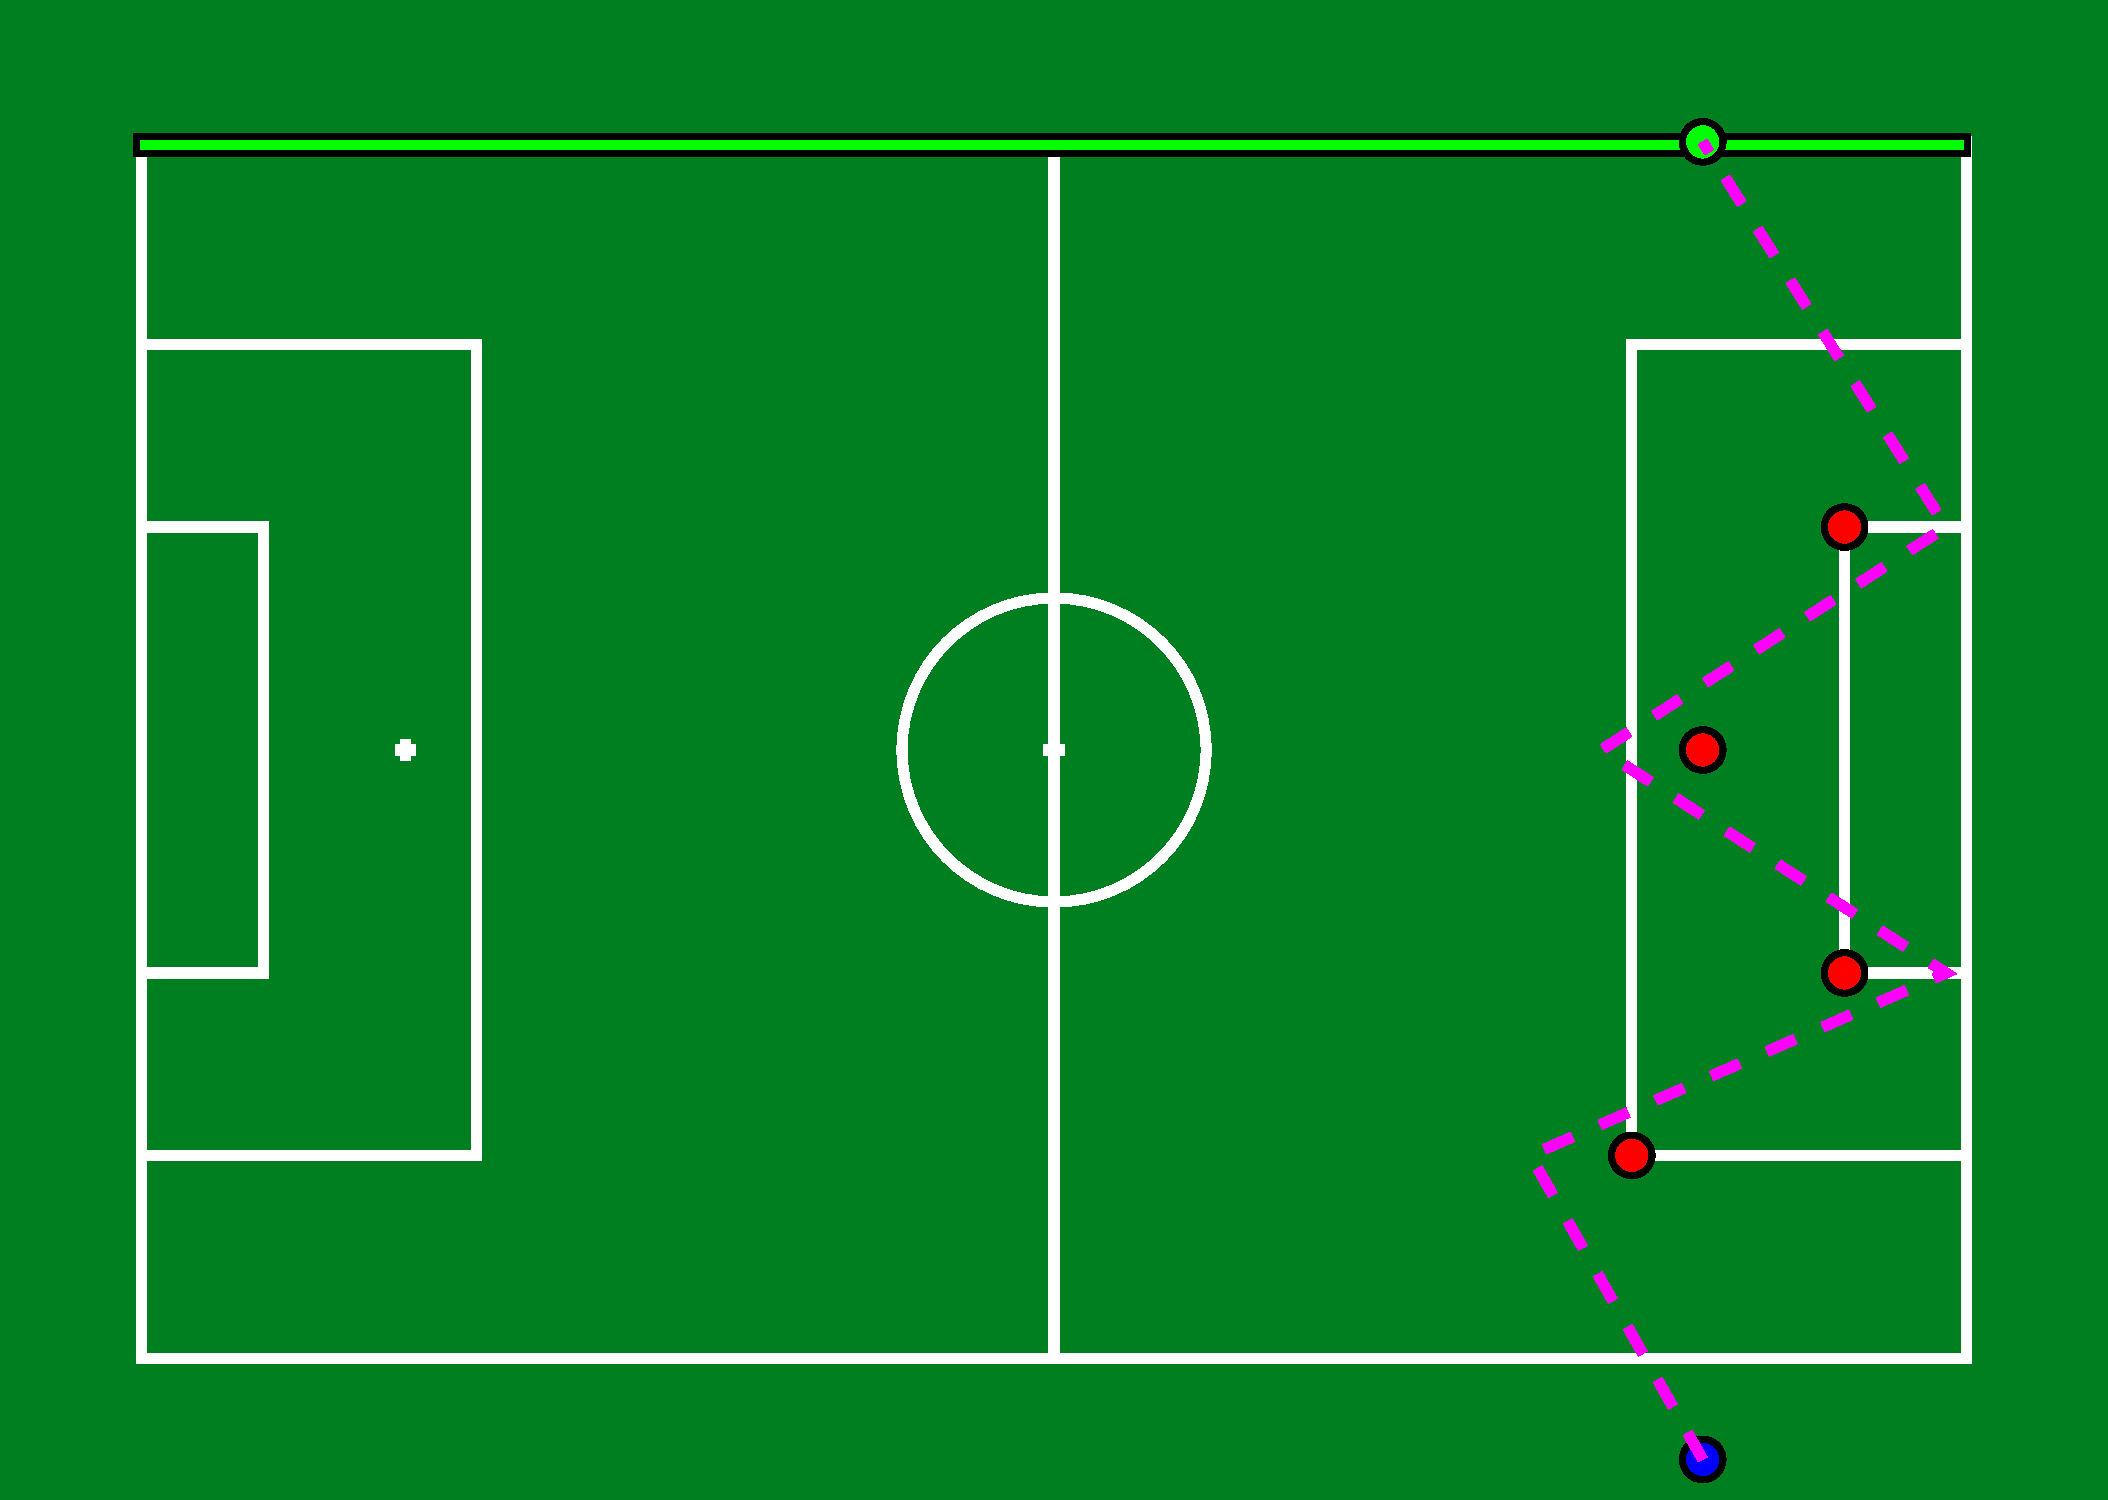
\includegraphics[width=\columnwidth]{figs/walk_leaderboard.pdf}}
    \caption{Fastest Walk Leaderboard: Robot completing the attempt is shown in blue, target is shown in green, obstacles are shown in red. An example path is shown in magenta}
    \label{fig:walk_leaderboard}
\end{figure}

\subsection{Challenge Execution}
Each attempt will consist of two types of runs, one with obstacles and one without.
Participating teams can choose which order they wish to complete these runs. Code changes are not allowed during an attempt,
but are allowed between attempts. The participating robot must navigate autonomously and cannot be remote controlled during the challenge.

\subsubsection{Obstacles}
Robots will be placed on the field as described above, the active robot will need walk from it's
starting position to the target touchline, while weaving around the obstacle robots. (see \cref{fig:walk_leaderboard} for an example)

\subsubsection{Open Field}
Robot obstacles will be removed from the field and the active robot will just need to walk 
from the starting position to the target touchline.

\subsection{Scoring}
Time starts once the robot touches the starting touchline and ends once the target touchline is touched

After all attempts, the shortest time to complete each type of run will be added together and recorded
on the leaderboard, times will be rounded to the nearest second.

\section{Best Kick Leaderboard}
This leaderboard will measure how far and how accurate a NAO will be able to kick a standard
SPL soccer ball.

\subsection{Setup}
This leaderboard challenge will take place on a standard SPL field, and requires 1 active robot and 1 ball.
The ball will be placed on the centre of the edge of the goal area.
The competing robot will be placed in the centre of the goaline facing the ball
\begin{figure}[t]
    \centerline{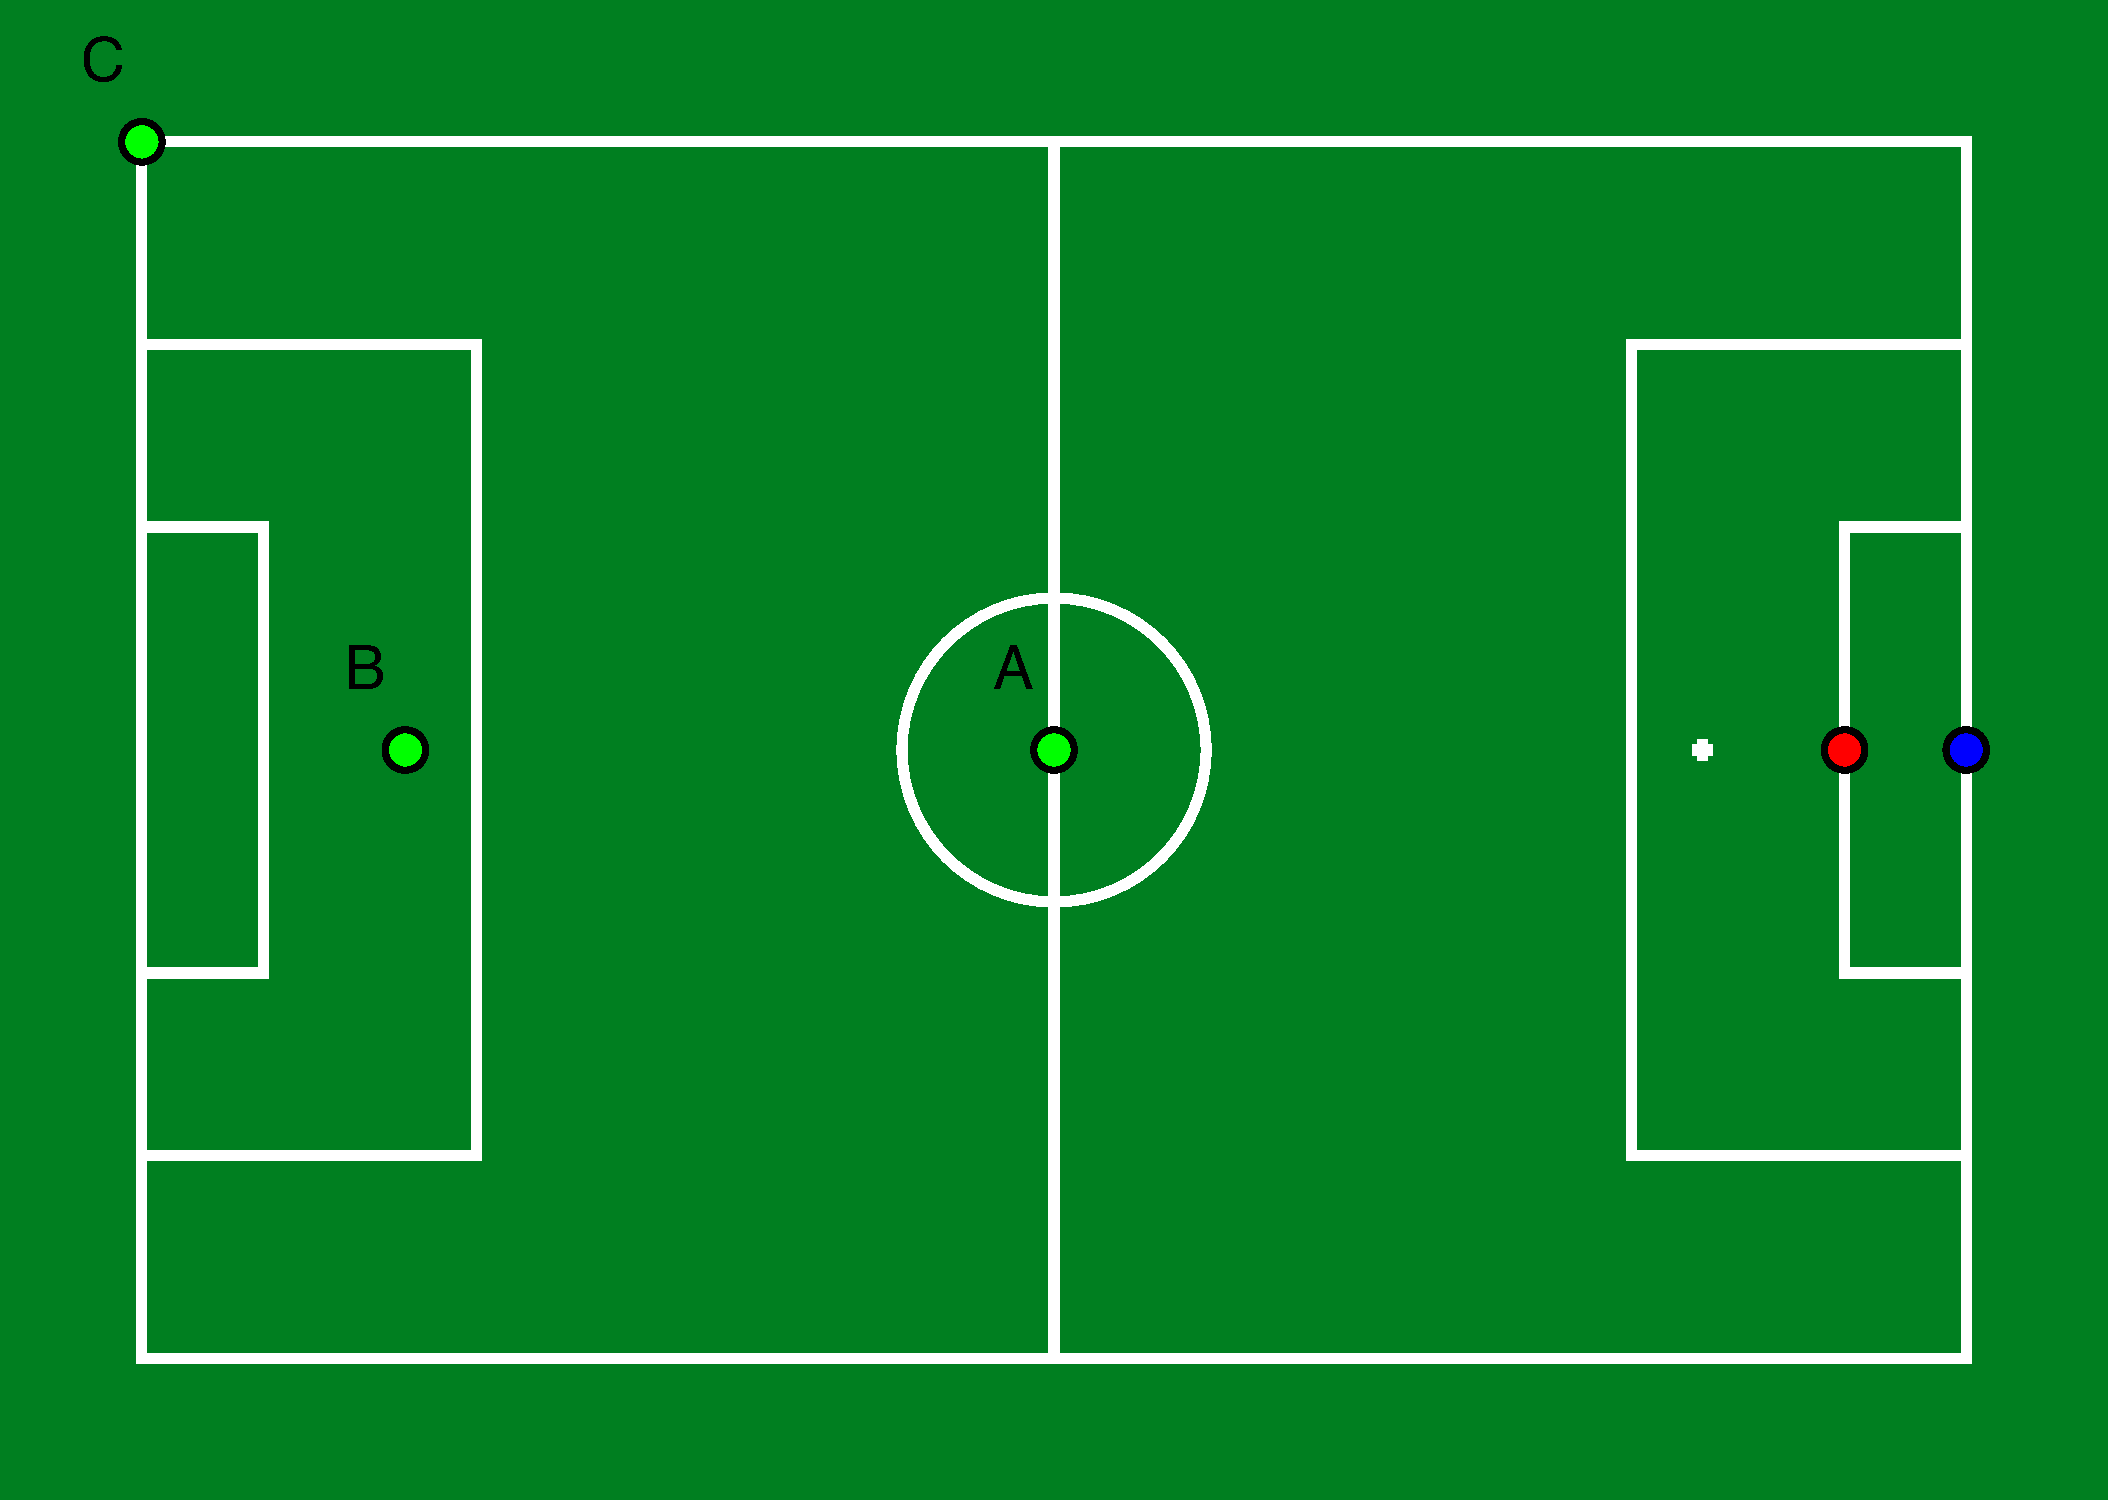
\includegraphics[width=\columnwidth]{figs/kick_leaderboard.pdf}}
    \caption{Best Kick Leaderboard: Robot completing the attempt is shown in blue, targets are shown in green, ball placement is shown in red}
    \label{fig:kick_leaderboard}
\end{figure}
\subsection{Challenge Execution}
Each attempt will consist of kicking towards each of the three targets (illustrated in \cref{fig:kick_leaderboard}):
\begin{itemize}
    \item The centre mark in the centre circle
    \item The penalty mark on the opposite side of the field
    \item A corner on the opposite side of the field
\end{itemize}
In each attempt, for each kick, participating teams must start the robot behaviour of their competing robot via a single chest button
press. The robot then has \qty{\PenaltyShootoutKickTime}{\second} to kick the ball towards the current target.
The competing robot must not touch the ball a second time after the ball has clearly moved,
otherwise the attempt ends immediately without scoring.
Once the ball has come to a complete stop, the distance from the ball to the target is measured.

Code changes are allowed when changing targets.
\subsection{Scoring}
After all attempts, the best score for each target will be added together and recorded in the leaderboard.
Distances are rounded to the closest centimetre.

\section{Most Passes Leaderboard}
This leaderboard measures the highest number of successful passes a team can
complete in a given timeframe, emphasizing passing accuracy, speed, and coordination.

\subsection{Setup}
This leaderboard challenge will take place on a standard SPL field and requires 2 competing robots,
a Game Controller and 1 standard SPL soccer ball.

Competing robots will be placed on the touchlines on opposite sides of the same half of the field,
in line with the penalty mark. The ball will be placed on either corner of the penalty area.

\begin{figure}[t]
    \centerline{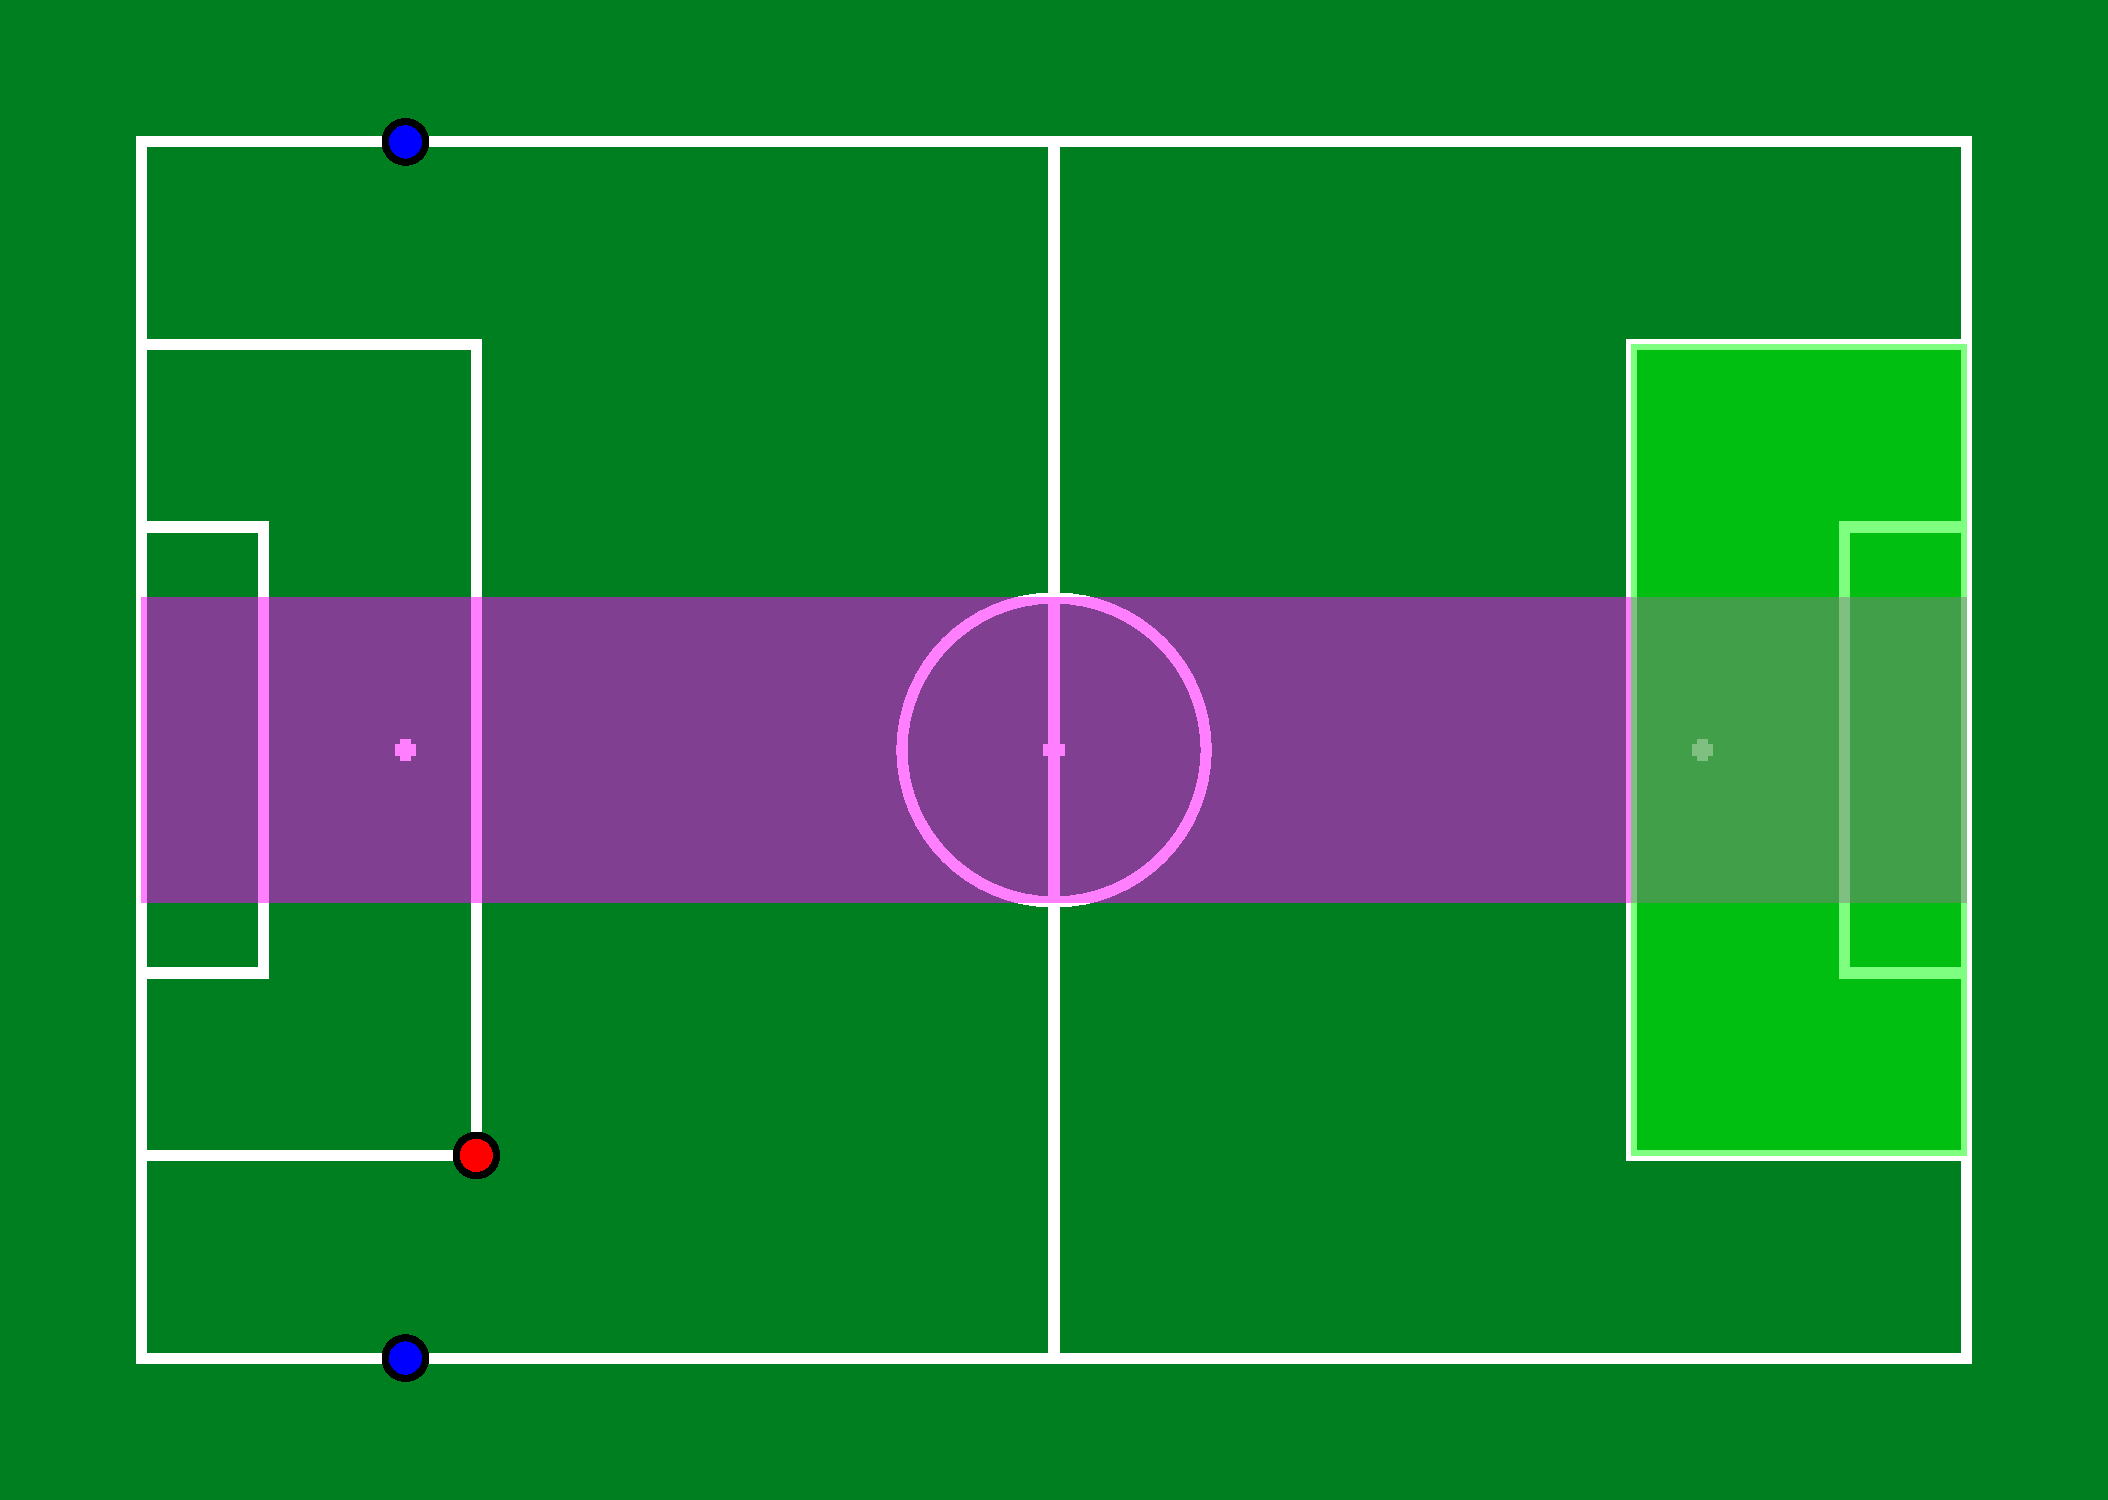
\includegraphics[width=\columnwidth]{figs/passing_leaderboard.pdf}}
    \caption{Passing Kick Leaderboard: Robots completing the attempt are shown in blue, target area is shown in green, exclusion area is shown in magents and ball placement is shown in red}
    \label{fig:passing_leaderboard}
\end{figure}
\subsection{Challenge Execution}
In each attempt, a playing packet will be sent from the game controller to indicate the start of the attempt,
and will begin counting down the timer.
Teams will then have at most \qty{\MaxTimePassingLeaderboard}{\sec} to move the ball from the starting
position to the target area while completing as many passes as possible. The centre
1.5 metres of the field (Centre Cricle Diameter) is an exclusion zone, no robots are allowed within this area,
if a robot enters this area, or the ball comes to a complete stop
within this area, the run is ended immediately. If the ball is kicked off the field,
it is placed back on the touchline where it crossed.

The ref will announce each time the ball crosses the exlusion zone, and whether this will
count as a successful pass. This is then captured by the Game Controller.

Once a robot has posession of the ball within the target area, the ref will announce that the
attempt has finished, then the finish signal will be sent from the game controller and the timer will stop.


\subsection{Scoring}
1 point is awarded every time the ball crosses the exlusion zone,
with an additional point awarded for a "successful pass". A "successful pass" is defined as when the
The ball stops in an 180◦ arc with radius 75cm in front of the receiving robot.

No points are counted if the time runs out before a robot has posession of the ball
within the target area, the ball hasn't crossed the exclusion zone at least once
or if the run ends prematurely as per the above rules.

The score is then multiplied by the number of seconds remaining on the game controller timer.

The highest score of all attempts will be recorded in the leaderboard.

\section{Ball Control Leaderboard}
This leaderboard will measure how well a NAO can keep control of a ball, while moving it
to a target.

\subsection{Setup}
This leaderboard challenge will take place on one half of a standard SPL field, and requires 1 active robot, 4 inactive robots and 1 SPL Soccer Ball.
Inactive robots will act as obstacles for the attempt and will be placed as follows (illustrated in \cref{fig:walk_leaderboard}):
\begin{itemize}
    \item On the penalty mark
    \item On both corners of the goal area that are not touching the field boundary
    \item On the corner of the goal area closest to the competing robot
\end{itemize}
The ball is placed on the touchline in line with the penalty mark, with the competing
robot placed around 50cm behind it.
The end goal is the touchline on the other side of the field.

\begin{figure}[t]
    \centerline{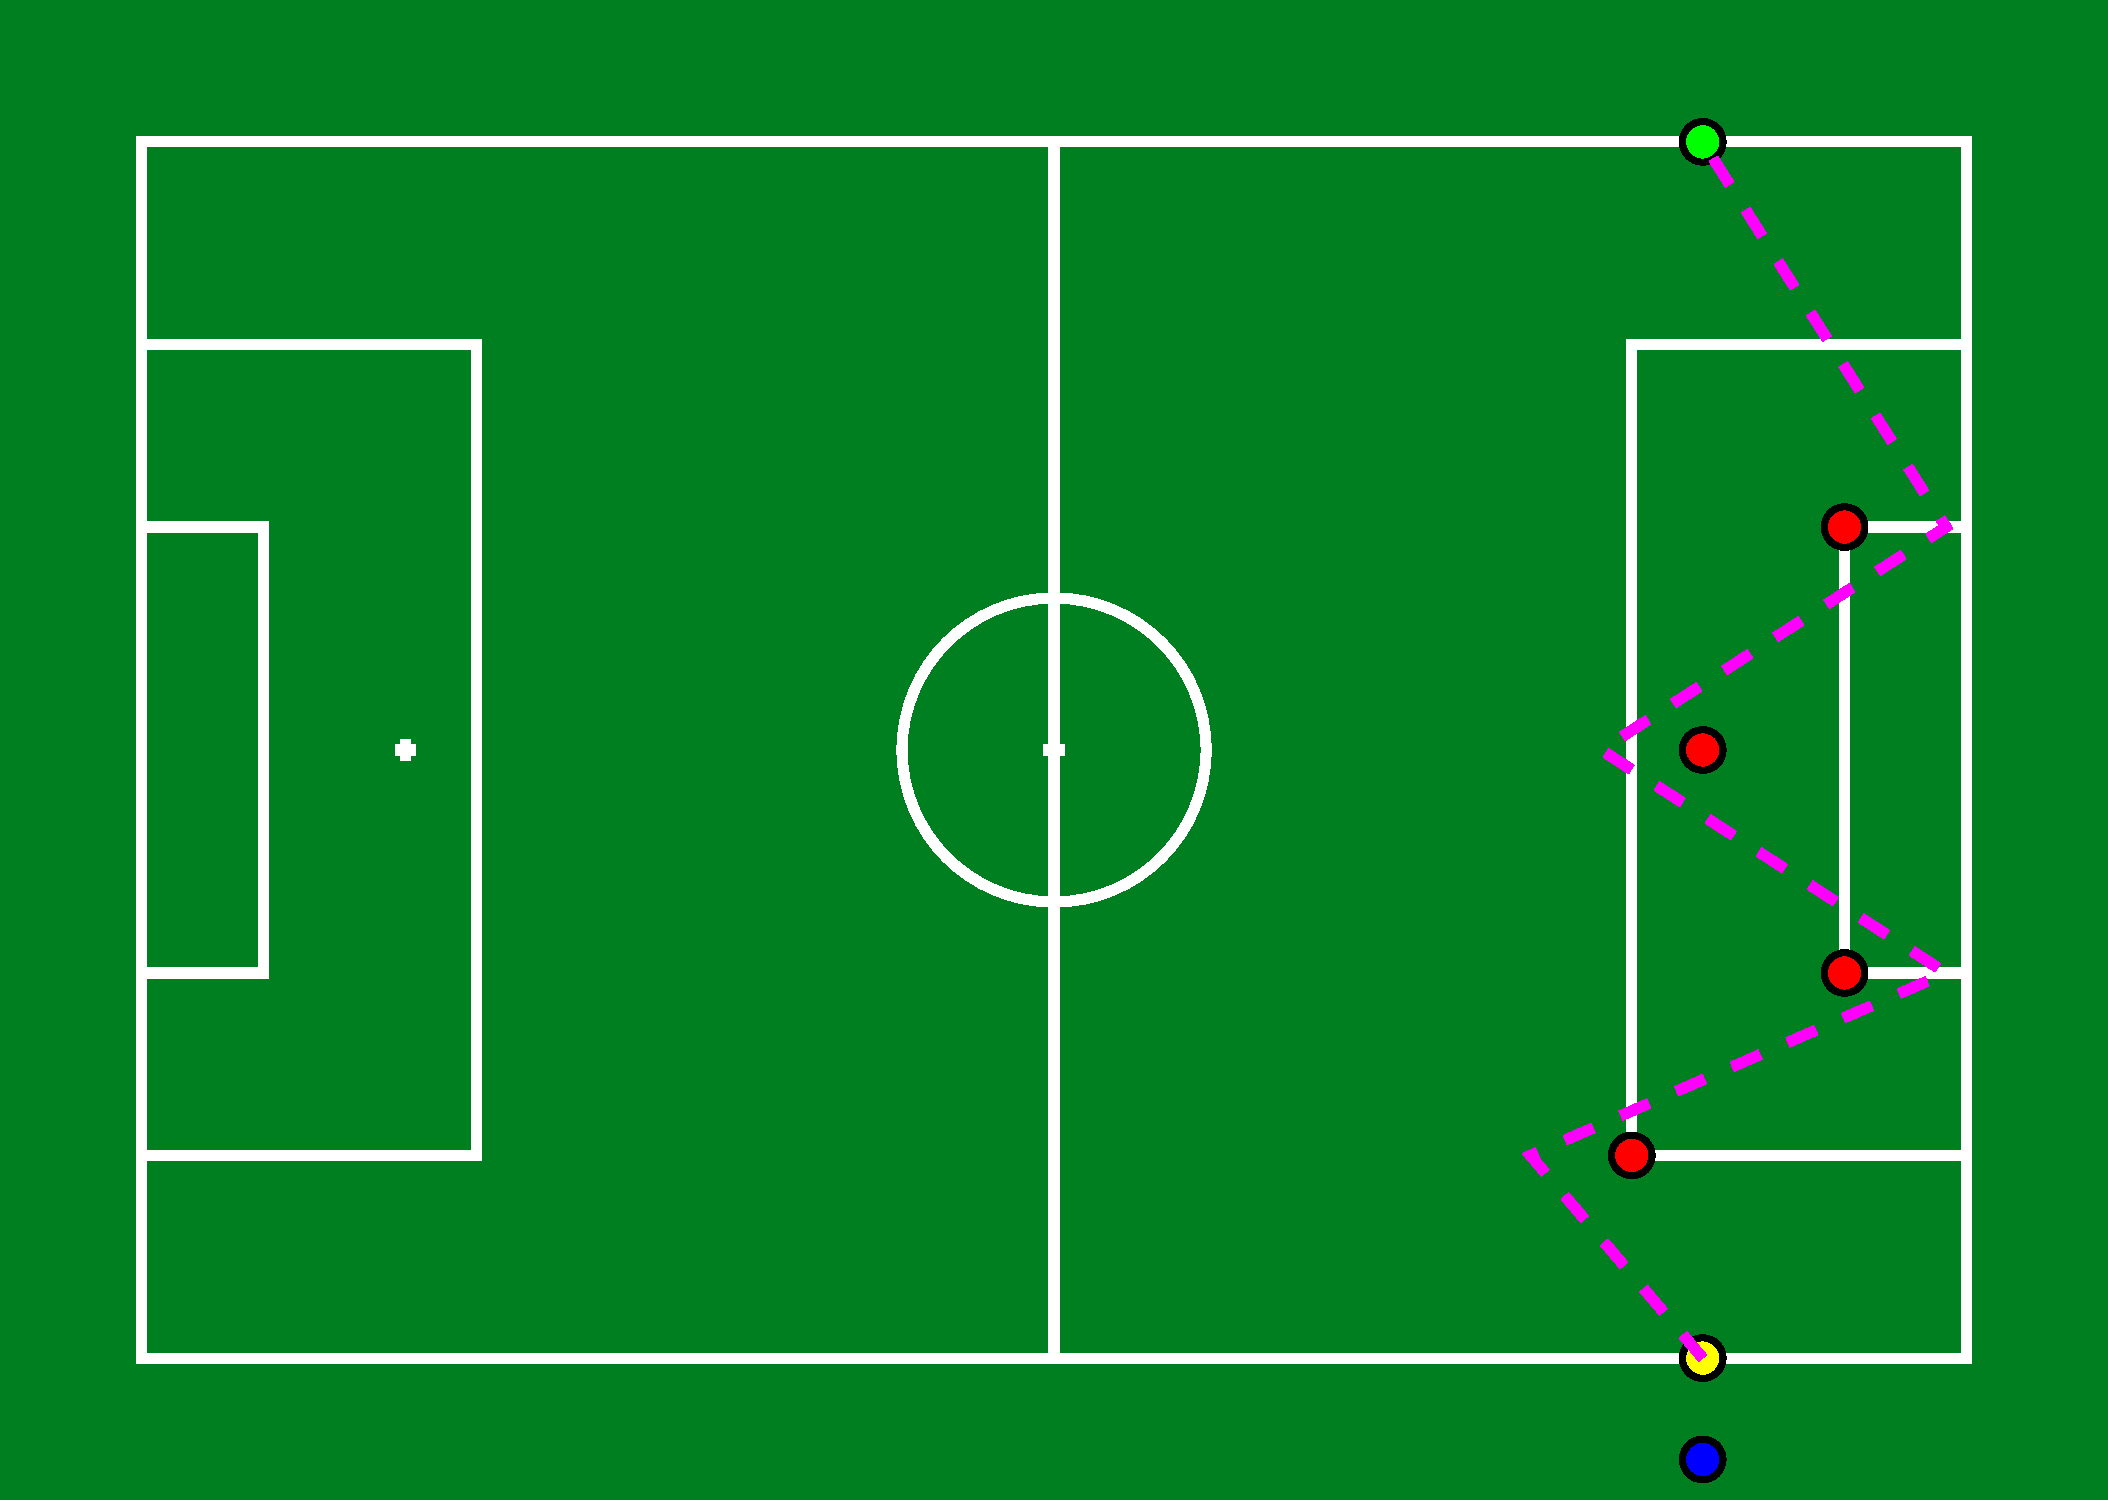
\includegraphics[width=\columnwidth]{figs/control_leaderboard.pdf}}
    \caption{Ball Control Leaderboard: Robot completing the attempt is shown in blue, target is shown in green, obstacles are shown in red and the ball is shown in yellow. An example path is shown in magenta}
    \label{fig:ball_control_leaderboard}
\end{figure}

\subsection{Challenge Execution}
In each attempt, participating teams must start the robot behaviour of their competing robot via a single chest button
press. Participating robots will need to dribble the ball around the obstacles and across
the goal touchline in as fast a time as possible.

Anytime the ball moves more than 75cm away from the competing robot or the ball comes in contact with
an obstacle,  ``Penalty'' is called, and a 30 second penalty we be added to the teams score.

\subsection{Scoring}
Time starts from when the chest button is pressed, to when to robot and ball entirely crosses the target touchline.

The lowest time across all attempts will be recorded in the leaderboard, times will be rounded to the nearest second.

\section{Global Performance Factor}
In addition to skill-specific leaderboards, a Global Performance factor will be published,
this will be used to rank teams based on performance consistency and competitiveness across
various challenges and games. The Global Performance Factor will be calculated using the 
Glicko ratings in combination with other performance indicators and  will provide a dynamic
rating that adjusts based on team performance year-over-year
offering a comprehensive view of each team's standing in the league.

\subsection{Calculation}
TBD
